
%% bare_jrnl.tex
%% V1.4b
%% 2015/08/26
%% by Michael Shell
%% see http://www.michaelshell.org/
%% for current contact information.
%% This is a skeleton file demonstrating the use of IEEEtran.cls
%% (requires IEEEtran.cls version 1.8b or later) with an IEEE
%% journal paper.
%%
%% Support sites:
%% http://www.michaelshell.org/tex/ieeetran/
%% http://www.ctan.org/pkg/ieeetran
%% and
%% http://www.ieee.org/
%@@@@@@@@@@@@@@@@@@@@@@@@@@@@@@@@@@@@@@@@@


\documentclass[onecolumn,journal] {IEEEtran}

\usepackage{graphicx}
\usepackage{amsmath}
\begin{document}


\title{A summary \\ Latex\\ Gnuplot \\ Git  and\ Probabiriry} %@@@@@@@@

\begin{Large}
\author{by~Praphasri  Bidasak,~\IEEEmembership \\{\today  }} 

\end{Large}

\begin{titlepage}

\end{titlepage}

 \maketitle

\newpage
%page2 
\tableofcontents
\begin{Large}
 A simple guide to LaTex 
\newline
\newline
\end{Large}

1.The basic laout of a LaTex      \\                                                                                              							2.Title pahe \\
3. Structuring document \\
4. Use packages in LaTex to add more functions. \\
5. Using inline math embed formulas in text \\
6.Adding figures in LaTex \\
7. Generate a table of contents in LaTex \\
8.Tables in LaTex 
\newline
\newline
\begin{Large}
Gnuplot Sort Course\\
\end{Large}
 1. Introduction\\
2. Basic 2D Plots \\
3.Operators, Constants, and Functions
\newline
\newline
\begin{Large}
Git Short Course
\end{Large}

\newpage %page3

\begin{figure}

\begin{Large}
 A simple guide to LaTeX
\end{Large}
\newline
\newline
\begin{Large}
1.The basic layout of a LaTeX
\end{Large}
\newline
\newline
Creating documents with LaTeX is simple. In contrast to Word, you start off with a plain text file (.tex file) which contains LaTeX code and the actual content. The control statements tell LaTeX how your content should be formatted. Before the settings become apparent, the .tex file has to be compiled (translated) into a .pdf file. A basic example document can be created with the following code:\\
\begin{center}
\begin{tabular}{ |c| } 
 \hline

\textbackslash \ documentclass \{article\}\\
\textbackslash \ begin\{document\}\\
\textbackslash \ end\{document\} \\
 \hline

\end{tabular}
\end{center}
\begin{center}
Table. 1 \\
\end{center}
 Once  translated this code into a PDF document   
\textbackslash \ documentclass \{article\}\\
This specifies what sort of document you intend to write. After that, add
commands to influence the style of the whole document, or load packages
that add new features to the LATEX system. To load such a package you use
the command 
\newline
\newline
\textbackslash \ begin\{document\}\\
Now you enter the text mixed with some useful LATEX commands. At
the end of the document you add the
\newline
\newline
\textbackslash \ end\{document\} \\
It is invaluable for debugging. Sometimes  some complicated bit of TeX code that's going badly wrong but  can't figure out exactly where the error is (for example, beamer tends to report errors at the end of the frame - since that's when it encounters them - but the actual error is buried deep within it). Then putting \textbackslash  \ end \{document\} \\
\newline
\begin{Large}
2.Title page\\  %@@@@@@@@@@@@@@@@@
\end{Large}

\begin{Large}
Displaying the title of  document 
\end{Large}
\newline

To display the title of your document you have to declare its components in the preamble and then use some additional code: \\

\center
  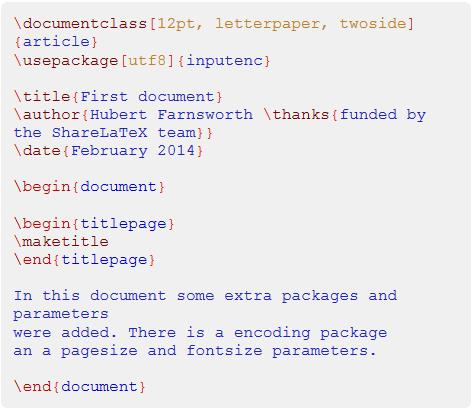
\includegraphics[width=8 cm]{code3.jpg}

% \caption{A boat.}

 % \labe{fig: boat1}

\end{figure}
\begin{center}
Figure.1 %PPPPPPPPPP
\end{center}
  
\begin{flushleft}
There is a block with three lines in the preamble that define what information is going to be included in the title page. \\

\textbackslash \ title\{First document\} 
\newline
This is the title.
\newline
\newpage
\textbackslash \  author\{Hubert Farnsworth\} 
\newline
 Here you put the name of the Author(s) and, as a optional parameter, you can add the next command: 
\newline
\newline
\textbackslash \ thanks \{funded by the ShareLaTeX team\}
This can be added after the name of the autor, inside the braces of the title command. It will add a superscript and a footnote with the text inside the braces. Useful if you need to thank an institution in your article. 
\newline
\newline
\textbackslash \ date\{February 2014\}
You can enter the date manually or use the command \today so the date will be updated automatically at the time you compile your document. \\


Once you have that in the preamble now in the body of your document you can use the next commands for the information to be printed. 
\newline
\newline
\textbackslash \ begin\{titlepage\}  \textbackslash \ end \{titlepage\}
This declares an environment, a block of code with a specific behaviour depending on its type. In this case whatever you include in this titlepage environment will appear in the first page of your document. 
\newline
\newline
\textbackslash \ maketitle \\ This command will print the title, the author and the date in the format shown in the example. If it's not enclosed in a titlepage environment, it will be shown at the beginning of the document, above the first line. 
\newline
\newline
\begin{Large}
3. Structuring  document - Adding paragraphs and sections
\end{Large}
\newline

Ccreated a very basic document in the previous lesson, but when writing a paper, it's necessary to structure the content into logic units. To achieve this, LaTeX offers us commands to generate section headings and number them automatically. The commands to create section headings are straightforward
\newline
\newline
Example output for section and subsection
The section commands are numbered and will appear in the table of contents of your document.\\
 Paragraphs aren't numbered and won't show in the table of contents. Here an example output using sections:
In order to get this output, we just have to add a few lines to our program 
\center
  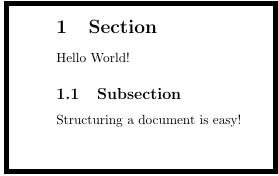
\includegraphics[width=5 cm]{dis5.jpg}


\begin{center}
Figure.2

\end{center}

\begin{flushleft}
Struturing a document LaTeX uses the commands
\newline

LaTeX uses the commands \textbackslash \ section \textbackslash   \ subsection and  \ textbackslash\ subsubsection to define sections in  document\\
The sections will have successive numbers and appear in the table of contents .
Paragraphs are not numbered and thus don't appear in the table of contents \\
\end{flushleft}

% \begin{flushleft}
\begin{center}

\begin{tabular}{ |c| } 

\hline
\newline
\textbackslash  \ begin\{document\}\\
\textbackslash   \ maketitle \\
 \textbackslash \ pagenumbering\{gobble\} \\
\textbackslash  \ newpage \\
 \textbackslash \ pagenumbering\{arabic\} \\  
 \textbackslash  \ pagenumbering  \ section\{Section\} \\
Hello World! \\
\textbackslash \ pagenumbering  \ subsection\{Subsection\} \\
 Structuring a document is easy! \\
\textbackslash \ pagenumbering \ pagenumbering\\  
\textbackslash \ end\{document\} \\
 \hline

\end{tabular}
\end{center} 

\begin{center}
Table. 2
\end{center}
%\newline
%\newline
\end{flushleft}

\begin{Large}
4. Use packages in LaTeX to add more functions. 
\end{Large} \\

There are countless packages, all for different purposes in my tutorials I will explain some of the most useful. To typeset math, LaTeX offers (among others) an environment called equation. Everything inside this environment will be printed in math mode, a special typesetting environment for math. LaTeX also takes care of equation numbers for us: \\
\begin{Large}
\newline
Including a package\\
\end{Large} \\
The automatic numbering is a useful feature, but sometimes it's necessary to remove them for auxiliary calculations. LaTeX doesn't allow this by default, now we want to include a package that :\\

\center
  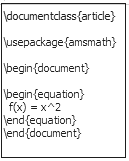
\includegraphics[width=4 cm]{uespack1.png}

\begin{center}
Table.3
\end{center}
\begin{flushleft}
Output as before, only the equation number is removed: $f(x) = x^2$ 
\newline
\newline
\begin{Large}
5. Using inline math - embed formulas in your text
\newline

The equation and align environment 
\end{Large} \\
The most useful math envorinments are the equation environment for typesetting single equationsand the align environment for multiple equations and automatic alignment
\end{flushleft}


\begin{flushleft}
The align environment will align the equations at the ampersand \&. Single equations have to be seperated by a linebreak 
There is no alignment when using the simple equation environment. Furthermore it is not even possible to enter two equations in that environment, it will result in a compilation error. The asterisk (e.g. equation*) only indicates, that I don't want the equations 
to be numbered 
\end{flushleft}

\center

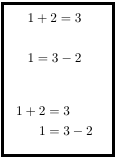
\includegraphics[width=4 cm]{dismat1.png}
\begin{center}
Figure.3
\newpage
\end{center} 
\begin{flushleft}
\begin{Large}
Fractions and more
\end{Large} 
\newline
\newline
LaTeX is capable of displaying any mathematical notation. It's possible to typeset integrals, fractions and more. Every command has a specific syntax to use. I will demonstrate some of the most common LaTeX math features:
\end{flushleft}
\center

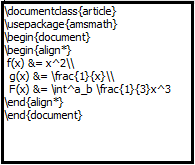
\includegraphics[width=5cm]{codemat2ee.png}
\begin{center}
Table.4
\end{center} 
\begin{flushleft}
\begin{Large}
Output:
\end{Large}
\end{flushleft}

\center
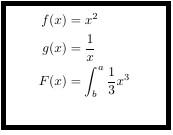
\includegraphics[width=5cm]{dismat2.png}
\begin{center}
Figuer.4
\end{center} 

\begin{flushleft}
\begin{Large}
6. Adding figures in LaTeX 
\end{Large} 
\newline

From time to time, it's necessary to add pictures to your documents. Using LaTeX all pictures will be indexed automatically and tagged with successive numbers when using the figure environment and the graphicx package.
\end{flushleft}

\center
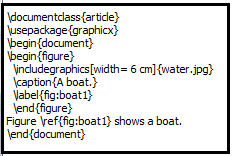
\includegraphics[width=6cm]{codepig1.png}
\begin{center}
Table.5
\end{center} 

\begin{flushleft}
\begin{Large}
The code above will create the following pdf: 
\end{Large} 
\end{flushleft}
\center
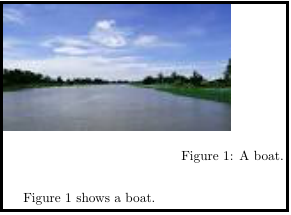
\includegraphics[width=5cm]{dispig1.png}
\begin{center}
Figure.5
\end{center} 
\newpage
\begin{flushleft}

The figure environment takes care of the numbering and positioning of the image within the document.
In order to include a figure, you must use the  |  includegraphics command. It takes the image width as an option in brackets and the path to your image file.can see, I put  | linewidth into the brackets, which means the picture will be scaled to fit the width of the document. As a result smaller pictures are upscaled and larger pictures downscaled respectively. As I mentioned before the brackets contain the path to the image. In this case the image is stored in the same directory as my .tex file, so I simply put boat.jpg here to include it. 
For large documents, you probably want to store image files in a different folder, say we created a folder images, then we would simply write images/boat.jpg into the braces. In the next command we set a | caption, which is the text shown below the image and a \label which is invisible, but useful if we want to refer to our figure in our document. You can use the \ref command to refer to the figure (marked by label) in your text and it will then be replaced by the correct number. LaTeX is smart enough to retrieve the correct numbers for all your images automatically. Note that you will need to include the graphicx package in order to use this code.
\newline
\newline
\begin{Large}
7. Generate a table of contents in LaTeX 
\end{Large}
\newline
\newline
Generating a table of contents can be done with a few simple commands. LaTeX will use the section headings to create the table of contents and there are commands to create a list of figures and a list of tables as well \\
The generation of a list of figures and tables works the same way. I added a dummy figure and table and put the lists in the appendix of my document:
\end{flushleft}

\begin{center}

\begin{tabular}{ |c| } 

\hline

\newline

\textbackslash  \ begin\{document\}\\
\textbackslash   \ begin\{figure\}\\
 \textbackslash  \ caption\{Dummy figure\}\\
  \textbackslash  \ end \{figure\}\\
 \textbackslash \ begin\{table\}\\
%\textbackslash \ caption\ {Dummy table\}\\
\textbackslash \ end\{table\} \\
\textbackslash \ begin\{appendix\}\\
 \textbackslash \ listoffigures\\
 \textbackslash  \ listoftables\\
\textbackslash\ end\{appendix\}\\
\textbackslash\ end\{document\}\\
 \hline
\end{tabular}
\end{center} 

\begin{center}
Table. 6
\end{center}
\begin{flushleft}
Autogenerate a table of content using 
\end{flushleft}
\center
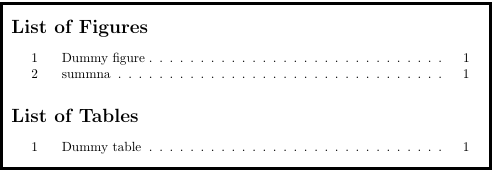
\includegraphics[width=8cm]{dislishof.png}
\begin{center}
Figure.6
\end{center} 
\begin{flushleft}
Autogenerate a table of content using  |tableofcontents\\
Create lists of your figures and tables with  | listoffigures and | listoftables\\
Always compile twice to see the changes
\newline
\newline
\begin{Large}
8.Tables in LaTeX 
\end{Large}
\newline
\newline
Try out all the features of LaTeX tables yourself. There's a huge list of code examples for tables somewhere on Wikibooks, which vast amount is almost overwhelming. As I mentioned before, it's usually faster to use a tool like excel to format your content and then let the pgfplots package autogenerate a table .


\end{flushleft}
\newpage
\center
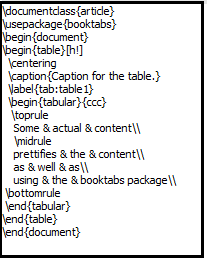
\includegraphics[width=5cm]{codetable1.png}
\begin{center}
\end{center} 

\begin{center}
Table. 7
\end{center}
\begin{flushleft}

There are two disadvantages of writing tablesWhile it works for small tables similar to the one in our example, it can take a long time to enter a large amount of data by hand. Most of the time the data will be collected in form of a spreadsheet and we don't want to enter the data twice. Furthermore once put into LaTeX tables, the data can not be plotted anymore and is not in a useful form in generalBut let's stick with writing tables by hand for now. The table above does not look very appealing. For this reason, we're now going to use the booktabs package to change this pitiful situation. The table we're going to get will be much nicer than before. Have a look at this:
 \end{flushleft}

 \center
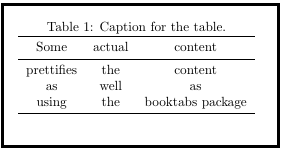
\includegraphics[width=7cm]{distable1.png}
\begin{center}
\end{center} 
\begin{center}
Figure.7
\end{center}
\begin{flushleft}
The code requires just a few changes.  used the following code to get this result:\\
LaTeX offers the table and tabular environment for table creation\\
The table environment acts like a wrapper for the tabular similar to the figure environment\\
Alignment and vertical separators are passed as an argument to the tabular   environment  ( begin{tabular})\\
It's possible to align the content left (l), centered (c) and right (r), where the number of alignment operators has to match the desired number of columns \\
The columns can be seperated by adding | in between the alignment operators\\
Rows can be seperated using the | hline command and columns using the ampersand   symbol 
\newline
\newline
\begin{Large}
 Gnuplot Short Course 
\newline
\newline
1.Introduction \\
\end{Large}
Gnuplot was originally developed by Colin Kelley and Thomas Williams in 1986 to plot functions and data
les on a variety of terminals. In 1988 and 1989 I created an alternate version, known as GnuTEX, that
supported a new |terminal type called latex, so gnuplot would output LATEX code. The plot could then be
included in a LATEX document. I added a number of embellishments, supported only by the latex terminal,
allowing the user to produce publication-quality plots.\\
Gnuplot is a powerful frccware program for plotting both 2D and 3D data Gnuplot will run under a variety of environments including Linux L,IRLX, Solaris, Windows. and DOS.\\
Should use this document in conjunction with "gnuplotcourse.tar.gz, an archive file that contains all of the scripts and data in this document (as well as the document itsilf) Form MI net machines.
\newline
\newline
\begin{Large}
1.Basic 2D Plots 
\end{Large} \\
To start guplot (make sure you are in the "data" directory first)'  simply type unix% gnuplot  and away  you go \\
Say you have a single column of data in a file called "1ch.dat" that you woule liked to plot\\
28.062\\
52.172\\
55.703\\
64.281\\
43.438, etc.\\
This is simple to plot\\
gnuplot will autoscale axes to include all the data. Bydefault, gnuplot will plot the data using points. The file '1ch.dat' must be in the current working directory that you ran gnuplot from, else you will have to specify the path to the file .../ and backslash are allowed

  gnuplot \textgreater   plot  '1ch.dat' \\ %@@@@@@@@@@@@@@@@@

 \end{flushleft}
 \center
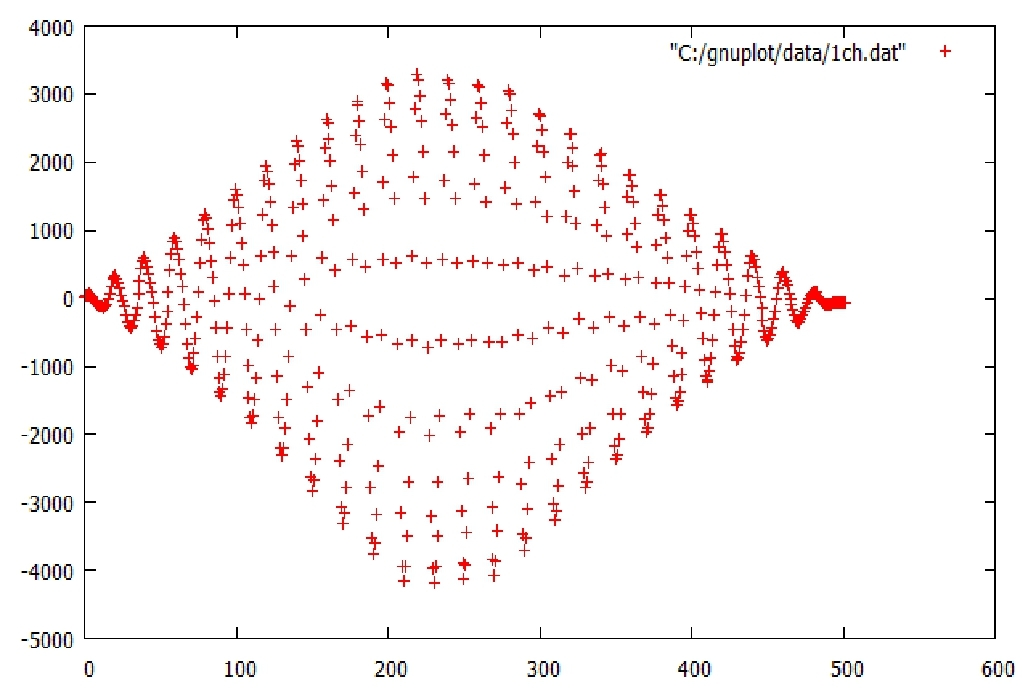
\includegraphics[width=8cm]{1ch.jpg}
\begin{center}
\end{center} 
\begin{center}
Figure.8
\end{center}
\begin{flushleft}
Let's plot the data  using lines, add more divisions to the xaxis, and rescale using set xrange.\\
 gnuplot \textgreater  set data style lines\\
 gnuplot \textgreater  set xtics 0,50,1000\\
gnuplot \textgreater  set  xrange[0:500]\\
gnuplot \textgreater  plot '../ data /textslash 1ch.dat' \\
\end{flushleft}
 
 \center
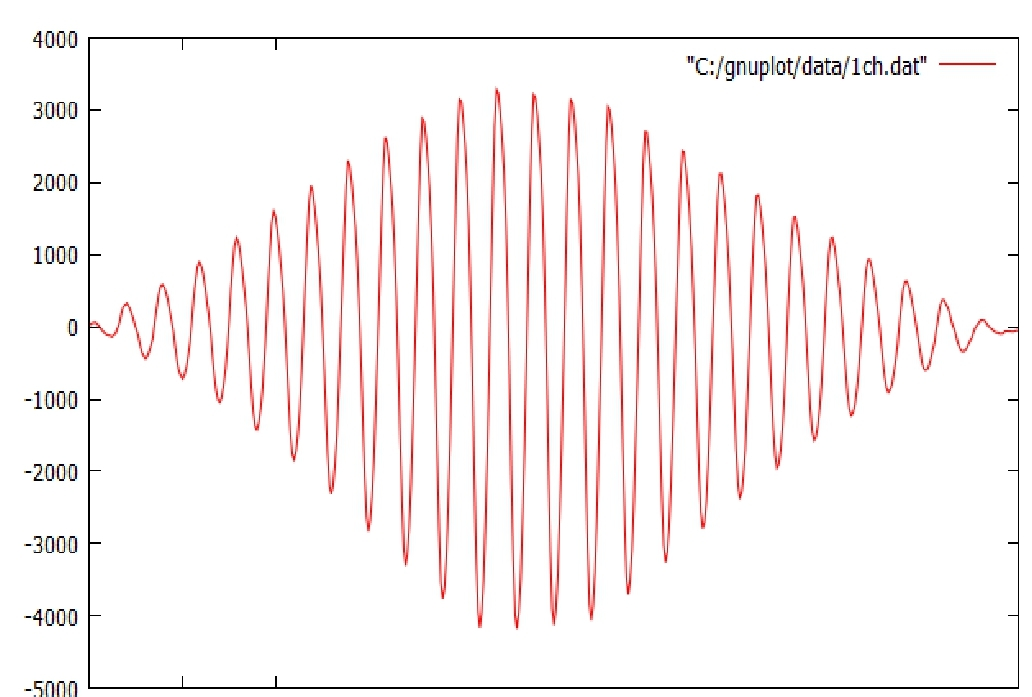
\includegraphics[width=8cm]{3ch.jpg}
\begin{center}
\end{center} 
\begin{center}
Figure.9
\end{center}
\begin{flushleft}
Ther are  several choices for data style. including lines, points, linespoints, or dots. The set xtics command takes three arguments,   \\
  \textless      start    \textgreater     ,     \textless    increment  \textgreater    ,    \textless end  \textgreater   ,and set xranger, two, 
    [\textless     start  \textgreater  :  \textless  end  \textgreater] .  
But what if you have multicolumn data? Is it possible to plot one column data? Of course! Gere we plot the second  column of data from the file "3ch.dat"\\ 
gnuplot \textgreater plot '3ch.dat' using 2 \\
The using command specifics a certain column of data, or cross-plots between coluns. Here we'll plot column l on the x-axis aand column 2 on the y.
\newline
\newline
gnuplot  \textgreater plot '3ch.dat' using 1:2
\end{flushleft}
 \center
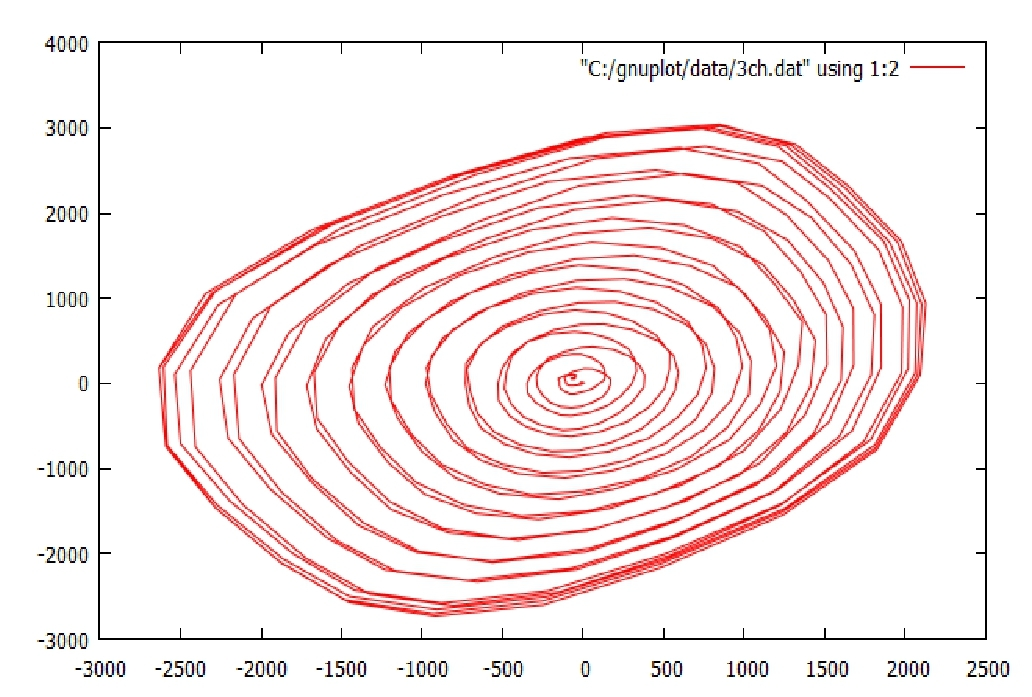
\includegraphics[width=8cm]{sinx.jpg}
\begin{center}
\end{center} 
\begin{center}
Figure.10
\end{center}
\begin{flushleft}
\begin{Large}
Operators, Constants, and Functions \\
\end{Large}
Gnuplot not only reads data fro files, it can also plot analytical functions. Toward thes cnd, gnuplot provides the  usual list of operatiors +, -,*,/, **, etc, and functions,sin(), cos(), log(), exp(), etc, A summary of operators and functions is available at the end of this text. Lext. Let's plot a simple function based on the above (note  that ** is exponentiation a la FDRTRAN).
\newline
gnuplot  \textgreater  set  xrange [0:250]\\
gnuplot  \textgreater  set(x) * (x**2)\\
Gnuplot assumes that x is  the independent variable. 
\end{flushleft}
 \center
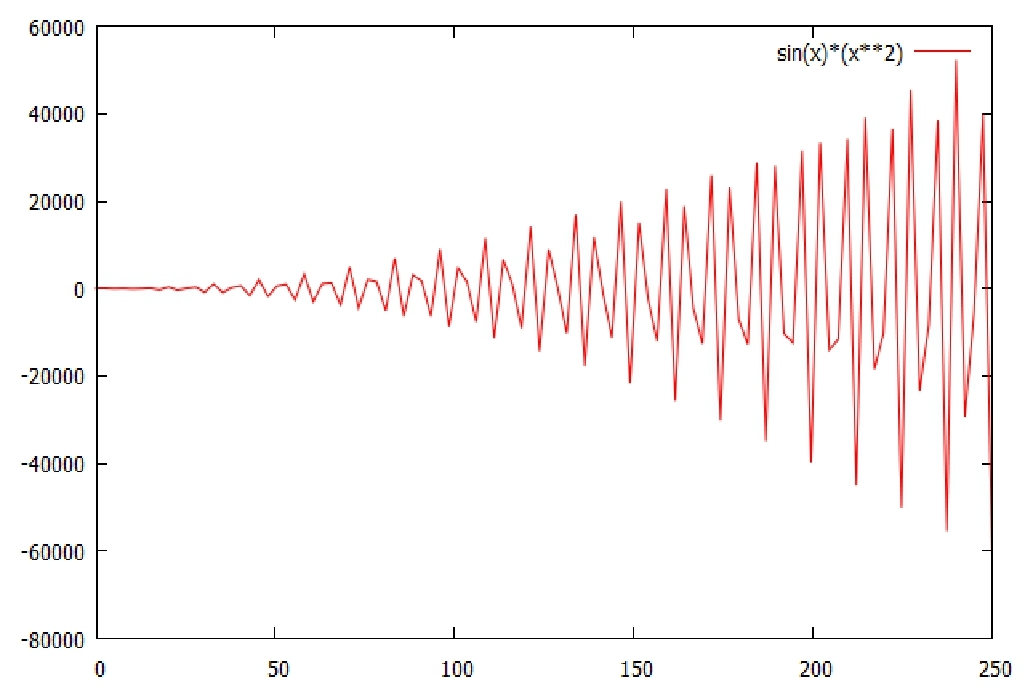
\includegraphics[width=8cm]{sinx1.jpg}
\begin{center}
Figure.11
\end{center}
\begin{flushleft}
The graph does not look like a sooth function at all. Gnuplot evaluatcs the function at  certain points only - the sample arte is too low for this function. Th change this, change\\
gnuplot  \textgreater  set  samples 1000 \\
gnuplot  \textgreater replot \\
\end{flushleft}

 \center
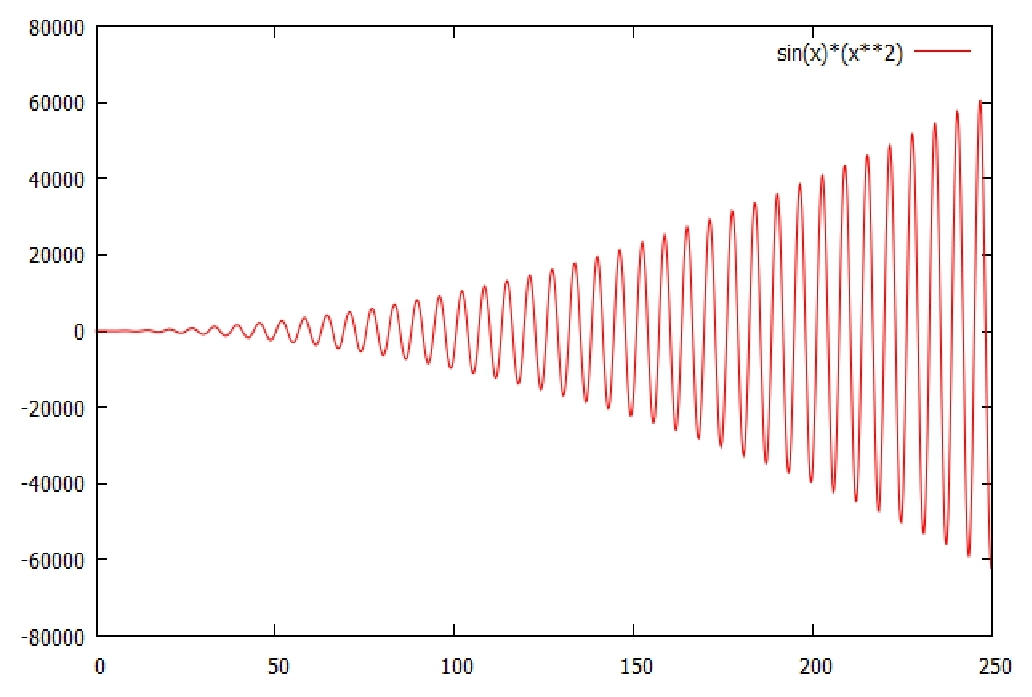
\includegraphics[width=8cm]{sinx3.jpg}
\begin{center}
 Figure.12
\end{center}

\begin{flushleft}
\begin{Large}
2. Gnuplot and LaTex
\end{Large}
\newline
\newline
If want to include gnuplot output in a Latex documemt, there are scveral options available. One gnuplot terminal type is latex. In this case, the output is   raw Latex code that can be included directly int a docuent. This has the advantage that LaTex is commands can be used in titles, etc.\\
gnuplot  \textgreater  set  xrange '$\epsilon$ (mm/mm)'\\
gnuplot  \textgreater  set ylabel '$\sigma$ (MPa)' \\
Gnuplot   \textgreater output 'plot.tex' \\
gnuplot  \textgreater  set  terminal latex \\
gnuplot  \textgreater  load 'script1.gp' \\
gnuplot  \textgreater set term x11 ; replot\\
\end{flushleft}

\center
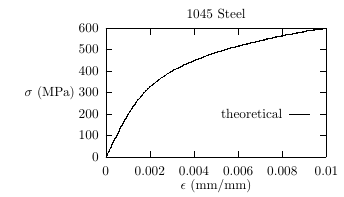
\includegraphics[width=9cm]{gnulatex.png}
\begin{center}
 Figure.13
\end{center}
\begin{flushleft}

The simplest way to include this in a Latex cocment is \\
\end{flushleft}
\begin{center}
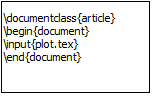
\includegraphics[width=5cm]{codein4.png}
\end{center}
\begin{center}
 Table.8
\end{center}

\begin{flushleft}
\begin{Large}
Git   Short Course
\end{Large}
\end{flushleft}



\end{document}
 



